
\section{Manual Patches}
Test
An image can have multiple discriminating patches. As shown in Figure \ref{fig:manual_patch}, some patches are highly noticeably discriminating such an open mouth and raised eyebrows in �surprise� expression or a wrinkled glabella (area between eyes) in �disgust� expression. Such patches can be the best approximation of most discriminating patches. Hence, they make a good basis for testing the algorithm. 

\begin{figure}
\centering
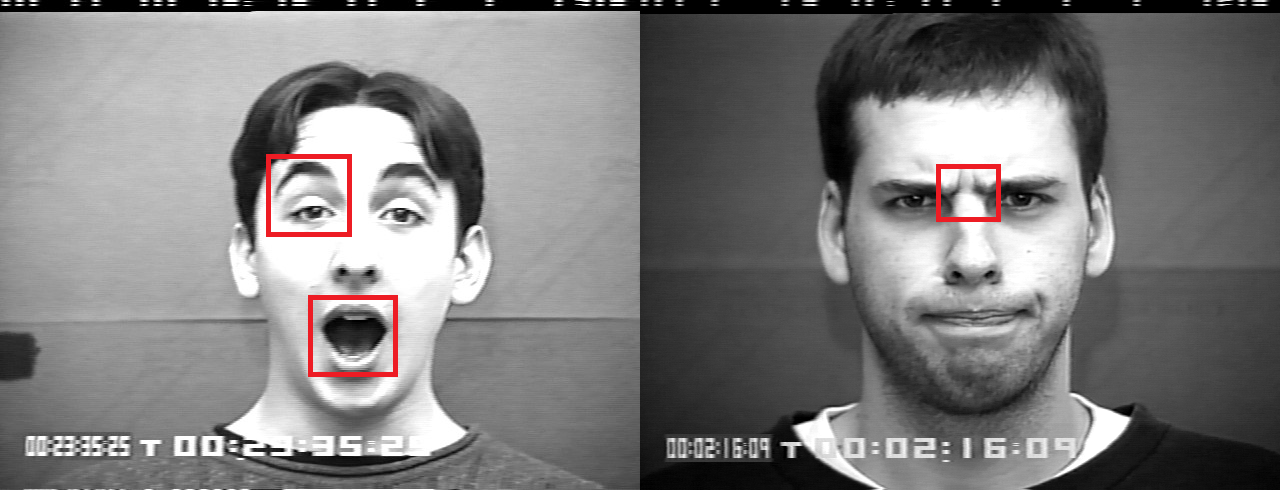
\includegraphics[width=300pt]{manual_patch.png}
  \caption{Noticeably discriminating patches}
  \label{fig:manual_patch}
\end{figure}

We identified four such patches, that 2 patches for eyes and one each for mouth and glabella. We extracted them manually and resized them to 36*36 pixels, 64*64 pixels and 96*96 pixels. It was ensured that extracted images of same patch are consistent with each other in terms feature content of the patch. For example, in case of mouth patches, it was ensured that the boundaries of the patch touch the edges of lips in all mouth patches.  


